\documentclass[a4paper,german,12pt,smallheadings]{scrartcl}
\usepackage[T1]{fontenc}
\usepackage[utf8]{inputenc}
\usepackage{babel}
\usepackage{geometry}
\usepackage{pdfpages}
\usepackage{tikz}
\usetikzlibrary{calc,intersections,fadings}
\usepackage{wrapfig}
\usepackage[fleqn]{amsmath}
\usepackage{amssymb}
\usepackage{float}
\usepackage{enumerate}
\usepackage{listings} % Source code
\usepackage{lscape} % landscape
\usepackage{commath} % http://tex.stackexchange.com/questions/14821/whats-the-proper-way-to-typeset-a-differential-operator
\usepackage{cancel}
\usepackage[fleqn]{mathtools}
\usepackage{xcolor}
\usepackage{pstricks}
\usepackage{pst-plot}
\usepackage{pst-math}
\usepackage{pst-pdf}
\usepackage{pstricks-add}
\usepackage[numbers]{natbib}
\usepackage{url}
% Number only referenced equations
%\mathtoolsset{showonlyrefs}

\usepackage{pgfplots}

%\usepackage{wrapfig}
\usepackage{siunitx}
\sisetup{separate-uncertainty=true,locale=DE}

% http://tex.stackexchange.com/questions/38818/best-way-to-denote-an-angle-in-tikz
\newcommand\markangle[6][red]{% [color] {X} {origin} {Y} {mark} {radius}
  % filled circle: red by default
  \begin{scope}
    \path[clip] (#2) -- (#3) -- (#4);
    \fill[color=#1,fill opacity=0.5,draw=#1,name path=circle]
    (#3) circle (#6mm);
  \end{scope}
  % middle calculation
  \path[name path=line one] (#3) -- (#2);
  \path[name path=line two] (#3) -- (#4);
  \path[%
  name intersections={of=line one and circle, by={inter one}},
  name intersections={of=line two and circle, by={inter two}}
  ] (inter one) -- (inter two) coordinate[pos=.5] (middle);
  % bissectrice definition
  \path[%
  name path=bissectrice
  ] (#3) -- (barycentric cs:#3=-1,middle=1.2);
  % put mark
  \path[
  name intersections={of=bissectrice and circle, by={middleArc}}
  ] (#3) -- (middleArc) node[pos=1.3] {#5};
  }

% New command for color underlining
\usepackage{xcolor}
\newcommand\invisiblesection[1]{%
    \refstepcounter{section}%
      \addcontentsline{toc}{section}{\protect\numberline{\thesection}#1}%
        \sectionmark{#1}}
\newsavebox\MBox
\newcommand\colul[2][red]{{\sbox\MBox{$#2$}%
  \rlap{\usebox\MBox}\color{#1}\rule[-1.2\dp\MBox]{\wd\MBox}{0.5pt}}}

\restylefloat{table}
\geometry{a4paper, top=15mm, left=20mm, right=10mm, bottom=20mm, headsep=10mm, footskip=12mm}
\linespread{1.5}
\setlength\parindent{0pt}
\DeclareMathOperator{\Tr}{Tr}
\DeclareMathOperator{\Var}{Var}
\begin{document}
\bibliographystyle{unsrt}

\begin{titlepage}
\newcommand{\HRule}{\rule{\linewidth}{0.5mm}}

\begin{center}
  \textsc{\Large Physikalisches Grundpraktkum 1}
  \HRule\\[0.4 cm]
  {\huge \bfseries Gleichmäßig beschleunigte Drehbewegungen}
  \HRule\\[0.4 cm]

  \begin{minipage}{0.65\textwidth}
  \begin{flushleft}
    Markus Fenske \texttt{<iblue@zedat.fu-berlin.de>} \\
    Paul Rahmann \texttt{<paulrahmann@zedat.fu-berlin.de>}
  \end{flushleft}
  \end{minipage}
  \hfill
  \begin{minipage}{0.30\textwidth}
  \begin{flushright}
    Tutor: Christian Hindermann \\
    Versuchstag: 6. Juni 2014
  \end{flushright}
  \end{minipage}

  \vspace{1cm}

  \tableofcontents


  %{\large \today}
  \vfill
\end{center}
\newpage

\end{titlepage}

\allowdisplaybreaks % Seitenumbrüche in Formeln erlauben

\section{Physikalische Grundlagen}
\subsection{Tunneleffekt}

\begin{figure}[h!]
  \centering
  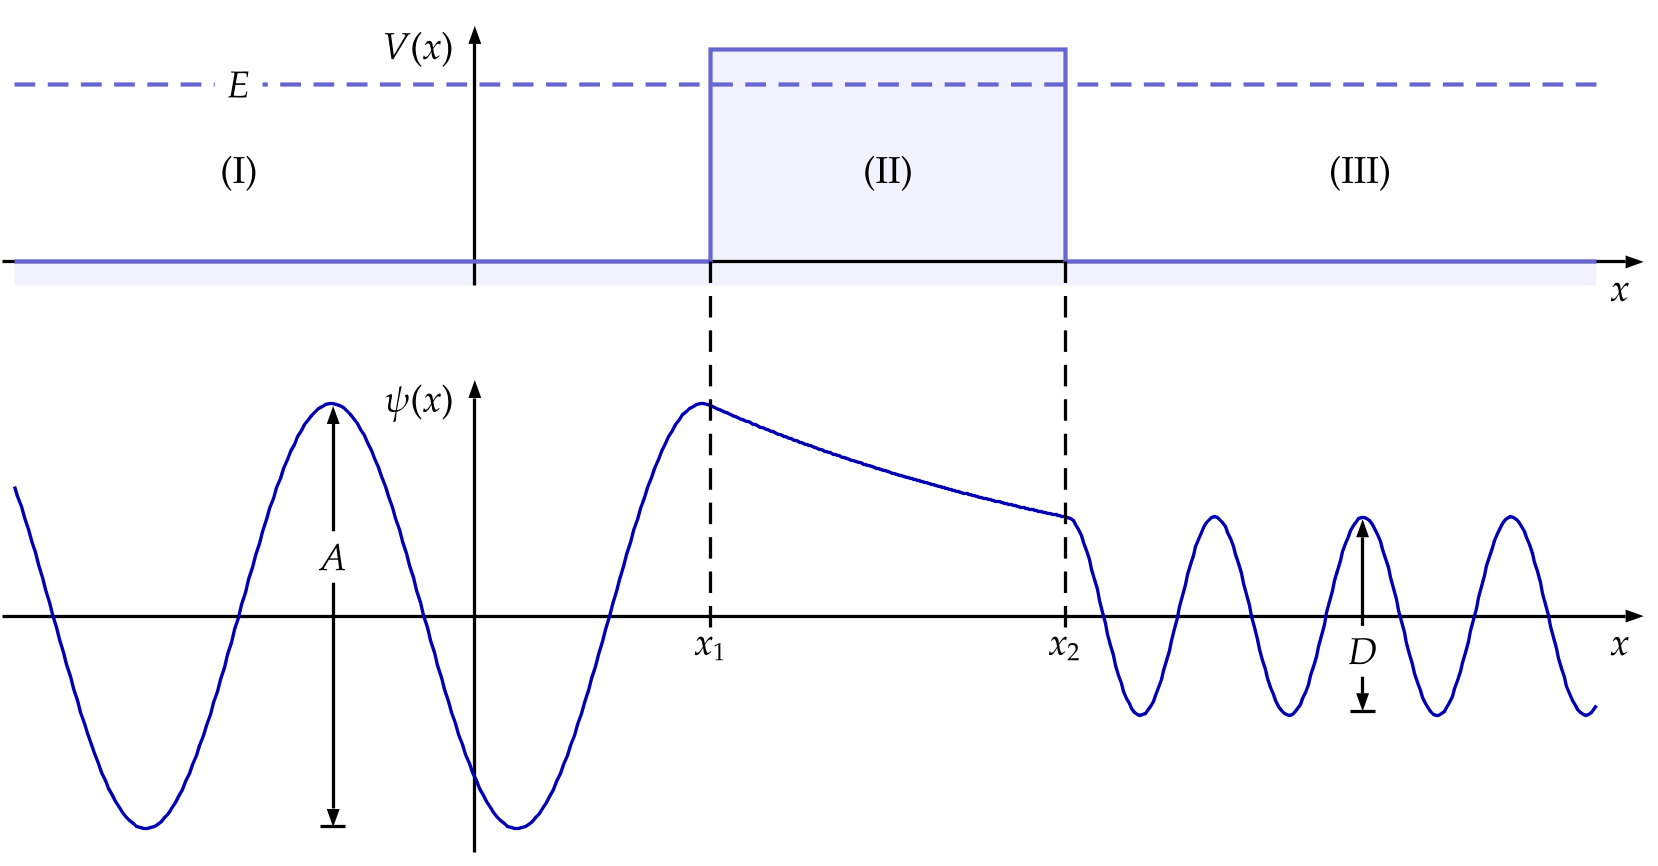
\includegraphics[width=1.0 \textwidth]{pic2.png}
  \caption{Lösung der Schrödingergleichung an einer Potentialstufe.\citep{pic2}}
\end{figure}

Gegeben sei ein Teilchen und eine Potentialstufe. Ist diese Potentialstufe
größer als die kinetische Energie des Teilchens, ist es dem Teilchen in
klassischer Betrachtung unmöglich, diese zu überwinden. In einer
quantenmechanischen Betrachtung gilt dies nicht mehr. Das Teilchen kann den
Potentialberg durchqueren. Man spricht veranschaulichend vom ``Tunneleffekt''.
Dieser ergibt sich direkt aus der Lösung der stationären eindimensionalen
Schrödingergleichung.

\begin{equation}
  \del{V - \frac{\hbar^2}{2m} \frac{\partial^2}{\partial x^2}} \Psi(x) = E \Psi(x)
\end{equation}

Wir betrachten ein kastenförmiges Potential.

\begin{equation}
  V(x) = \begin{cases} V_0 & \text{falls } x_1 \le x \le x_2 \\ 0 & \text{sonst} \end{cases}
\end{equation}

Wenn das Teilchen nun von $-\infty$ einläuft, erhalten wir drei verschiedene
stetig aneinander anschließende Lösungen

\begin{align*}
  \Psi_{I}(x) &= A e^{ikx} + B e^{-ikx} \\
  \Psi_{II}(x) &= C e^{\kappa x} + D e^{-\kappa x} \\
  \Psi_{III} &= F e^{ikx}
\end{align*}

mit den Koeffizienten

\begin{align*}
  k &= \sqrt{\frac{2mE}{\hbar^2}} \\
  \kappa &= \sqrt{\frac{2m (V_0 - E)}{\hbar^2}}
\end{align*}

Diese Modell lässt sich leider nur qualitativ auf das Rastertunnelmikroskop
übertragen. Beim Rastertunnelmikroskop wird eine Spitze im Abstand von wenigen
Angström über eine Probe gefahren. Zwischen Probe und Spitze wird eine Spannung
angelegt, das Potential ist somit in erster Näherung linear abfallend. Auch ist
das Problem nicht mehr als eindimensional zu betrachten. Um den Tunnelstrom
theoretisch vorherzusagen sind umfangreichere Betrachtungen nötig, so dass wir
hier nur das Ergebnis von \citep{hpa1982} wiedergeben wollen.

\begin{equation}
  I_{T} \propto \frac{V_T}{s} \exp \del{-A \phi^{1/2} s}
\end{equation}

Dabei ist $V_T$ die Tunnelspannung, $s$ der Abstand zwischen Probe und Spitze,
$A$ eine vom Zwischenraum abhängige Konstante und $\phi$ die Austrittsarbeit
aus der Probe an der gegebenen Stelle. Im Vakuum gilt
$A \approx 1{,}02 \AA^{-1} \text{eV}^{-1/2}$ nach \citep{versuchsanleitung}

\subsection{Piezoelektrischer Effekt}

Bestimmte Kristalle erzeugen bei Streckung oder Stauchung eine elektrische
Spannung. Dies ist dadurch erklärbar, dass sich durch die Verformung die
Schwerpunkte der positiven und negativen Ladungen verschieben. In den
Elementarzellen entstehen somit Dipole, die sich zu eine makroskopisch
messbaren Spannung aufsummieren. Umgekehrt entstecht durch Anlegen einer
Spannung eine Verformung. Dies wird im Rastertunnelmikroskop benutzt, um die
Spitze in sehr genauen Bereichen zu bewegen (rastern)\citep{versuchsanleitung}.

\subsection{Regelkreis}

Um den Tunnelstrom konstant zu halten, wird die Spitze der Probe bei einer
X-Y-Lageveränderung durch einen Regelkreis nachgeführt. Dazu wird der
tatsächliche Wert mit dem Sollwert verglichen und die Spitze entsprechend
bewegt.

\subsection{Tunnelspektroskopie}

Aus der X-Y-Spannung und der Z-Spannung erhält man durch zurückrechnen den
dreidimensiolen Ort der Spitze. Diese fährt die Äquipotentialflächen der
elektronischen Struktur der Probe ab, was Rückschlüsse auf die Probe erlaubt
(Tunnelspektroskopie).

\subsection{Räumliche Struktur von Festkörpern}

Festkörper im physikalischen bestehen aus sich periodisch wiederholenden
Strukturen. Das Modell geht dabei von einem unendlichen Kristall aus, der
translationssymmetrisch ist. Verschiebt man ihn um einen Gittervektor, erhält
man den Ausgangskristall. Festkörper lassen sich dabei gemäß ihrer
Gittervektoren in verschiedene Kristallsysteme einordnen.

Beim untersuchten Graphit handelt es sich um Lagen aus hexagonalen Kristallen.

\begin{figure}[h!]
  \centering
  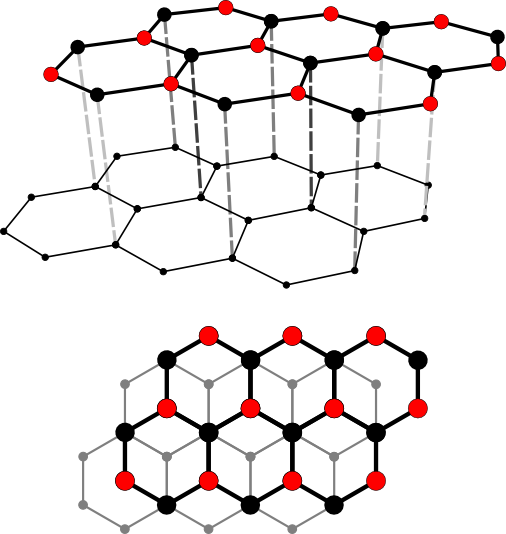
\includegraphics[width=0.6 \textwidth]{pic3.png}
  \caption{Grafitschichten in zwei verschiedenen Ansichten.\citep{pic3}}
\end{figure}

\subsection{Fouriertransformation}

Zur Analyse periodischer Strukturen ist die diskrete Fouriertransformation
geeignet. Dabei wird ein Datensatz $(a_0, a_1, \dots, a_{N-1})$ aus dem Ortsraum in
den Frequenzraum transformiert.

\begin{equation}
  \hat{a}_k = \sum_{j=0}^{N-1} \exp\del{2 \pi \text{i} \frac{jk}{N}} a_j
\end{equation}

Transformiert man das Signal so, erhält man die Frequenzkomponenten. Im
zweidimensionalen ist dies geeignet, um die reziproken Gittervektoren zu
erhalten.

\section{Auswertung}

\subsection{Aufgabe a}

Bearbeitet.

\subsection{Aufgabe b}

Zur Auswertung benutzen wir WSxM\cite{wsxm}
Die Topographiedaten wurden mit dem Filter ``Flatten'' geladen und anschließend
die ebenen Flächen mit dem Tool ``Local Plane'' markiert. Durch das Ziehen von
Linien mit dem Tool ``Profile'' haben wir die Höhenprofile durch die Stufen
haben wir die Durchschnittshöhe oberhalb und unterhalb der Stufe erhalten. Die
Fehler ergeben sich aus der Maximalabweichung nach oben und unten. Der Wert ist
der Durchschnittswert.

In der Numerierung ausgelassene Aufnahmen zeigten entweder den selben Bereich
wie die vorherige Aufnahme oder waren qualitativ nicht nutzbar. Sie wurden zur
Auswertung nicht herangezogen.

\vspace{5mm}
 \begin{tabular}{l|r|r|r}
  Quelle & Obere Ebene [\AA] & Untere Ebene [\AA] & Differenz [\AA] \\
   \hline
   $\texttt{HOPG\_\_0001.b.top}$ (a) & $\num{5.5+-1.0}$ & $\num{3.0+-2.0}$ & $\num{2.5+-2.3}$ \\
   $\texttt{HOPG\_\_0001.b.top}$ (b) & $\num{7.0+-3.0}$ & $\num{2.0+-2.0}$ & $\num{5+-3.7}$ \\
   $\texttt{HOPG\_\_0001.b.top}$ (c) & $\num{20+-6}$    & $\num{2+-6}$     & $\num{18+-8.5}$ \\
   $\texttt{HOPG\_\_0002.f.top}$ (a) & $\num{6+-2}$     & $\num{4+-3}$     & $\num{2+-3.7}$ \\
   $\texttt{HOPG\_\_0002.f.top}$ (b) & $\num{5.5+-1.5}$ & $\num{2.5+-1}$   & $\num{3+-1.9}$ \\
   $\texttt{HOPG\_\_0002.f.top}$ (c) & $\num{7.5+-1.5}$ & $\num{4.5+-1}$   & $\num{3+-1.9}$ \\
   $\texttt{HOPG\_\_0003.f.top}$ (a) & $\num{6+-1}$     & $\num{2.5+-3}$   & $\num{3.5+-3.2}$ \\
   $\texttt{HOPG\_\_0003.f.top}$ (b) & $\num{7+-1}$     & $\num{3+-3}$     & $\num{4+-3.2}$ \\
   $\texttt{HOPG\_\_0003.f.top}$ (c) & $\num{8+-1}$     & $\num{3+-3}$     & $\num{5+-3.2}$ \\
   $\texttt{HOPG\_\_0007.f.top}$     & $\num{8+-1}$     & $\num{2+-2}$     & $\num{6+-2.3}$ \\
   $\texttt{HOPG\_\_0008.b.top}$     & $\num{2+-2}$     & $\num{9+-1}$     & $\num{7+-2.3}$ \\
   $\texttt{HOPG\_\_0009.b.top}$     & $\num{3+-2}$     & $\num{9+-3}$     & $\num{6+-3.7}$ \\
   $\texttt{HOPG\_\_0010.f.top}$     & $\num{20+-20}$   & $\num{70+-20}$   & $\num{50+-29}$ \\
   $\texttt{HOPG\_\_0011.f.top}$     & $\num{4+-1}$     & $\num{2+-2}$     & $\num{2+-2.3}$ \\
   $\texttt{HOPG\_\_0012.b.top}$     & $\num{5+-5}$     & $\num{4+-6}$     & $\num{1+-7.9}$ \\
   $\texttt{HOPG\_\_0013.f.top}$ (a) & $\num{7+-7}$     & $\num{6+-4}$     & $\num{1+-8.1}$ \\
   $\texttt{HOPG\_\_0013.f.top}$ (b) & $\num{3+-3}$     & $\num{22+-5}$    & $\num{19+-5.9}$ \\
   $\texttt{HOPG\_\_0014.f.top}$     & $\num{2+-1}$     & $\num{72+-2}$    & $\num{70+-2.3}$ \\
   $\texttt{HOPG\_\_0015.b.top}$ (a) & $\num{1.5+-1}$   & $\num{8+-1}$     & $\num{6.5+-1.5}$ \\
   $\texttt{HOPG\_\_0015.b.top}$ (b) & $\num{14+-2}$    & $\num{8+-8}$     & $\num{6+-8.3}$ \\
 \end{tabular}
\vspace{5mm}

Im folgenden Plot sind die Daten aufgetragen. Es ist zu erkennen, dass die
Fehler viel zu groß sind, um irgendwelche Häufungen zu erkennen. Somit lässt
sich der Literaturwert von $3{,}35$ \AA weder bestätigen noch widerlegen. Eine
Überprüfung der Kalibrierung ist mit diesen Daten ebenfalls nicht möglich.

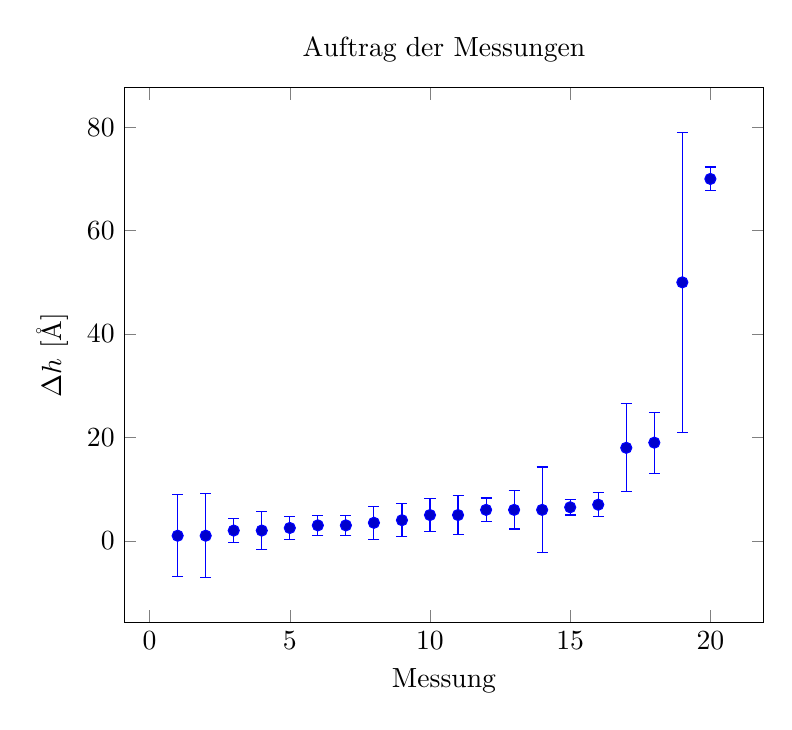
\begin{tikzpicture}
  \begin{axis}[
      width=0.8\textwidth,
      title=Auftrag der Messungen,
      xlabel={Messung},
      ylabel={$\Delta h$ [\AA]}
    ]
  \addplot+[only marks,error bars/.cd, y dir=both, y explicit]
  table[x=x,y=y,y error=err]
  {
    x y err
    1 1.0 7.9
    2 1.0 8.1
    3 2.0 2.3
    4 2.0 3.7
    5 2.5 2.3
    6 3.0 1.9
    7 3.0 1.9
    8 3.5 3.2
    9 4.0 3.2
    10 5.0 3.2
    11 5.0 3.7
    12 6.0 2.3
    13 6.0 3.7
    14 6.0 8.3
    15 6.5 1.5
    16 7.0 2.3
    17 18.0 8.5
    18 19.0 5.9
    19 50 29
    20 70 2.3
  };
  \end{axis}
\end{tikzpicture}

\subsection{Aufgabe c}

Während der Messung 16 fiel das STM aus. Da der Spannungsverstärker einen
Overdrive anzeigte, gingen wir davon aus, dass die Spitze in die Probe gefahren
war. Wir stellen zwei Mal eine neue Spitze und Probe her, konnten aber keine
stabile Messung mehr durchführen.

Wir haben allerdings Daten einer Referenzmessung erhalten, die wir im folgenden
auswerten.

\subsection{Aufgabe d}
Bei den auftretenden Strukturen handelt es sich, statt dem erwarteten
hexagonalen Gitter, um ein triagonales Gitter. Dies liegt darin begründet, nur
jedes zweite Atom sichtbar ist, da die unterliegende Schicht durch
van-der-Waals-Kräfte die elektronen ``absaugt''. Der Abstand zum jeweils
übernächsten Nachbarn ergibt sich dann aus geometrischen Überlegungen als
$2{,}46$ \AA.

Mithilfe der Software haben wir die Abstände in drei verschiedene Richtungen
anhand der Datei \texttt{Graphite\_\_0008.f.ch1} bestimmt (siehe Abbildung).
Dazu haben wir jeweils Profillinien parallel zu den Gittervektoren erstellt und
die Anzahl der Peaks entlang der Linien gezählt.  Bei den Längen haben wir als
Fehler eine halbe Peakbreite angenommen. So erhalten wir die Gitterkonstanten
in verschiedenen Richtungen.

\begin{figure}[h!]
  \centering
  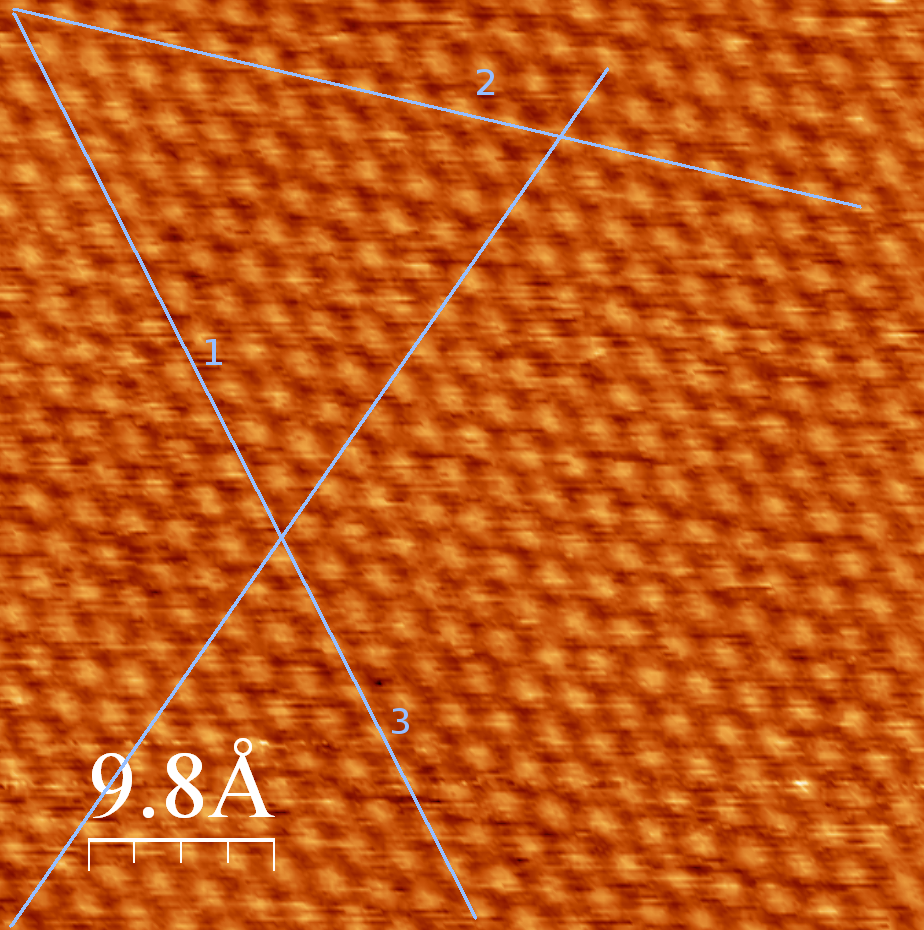
\includegraphics[width=0.5 \textwidth]{atomic.png}
  \caption{Messrichtungen}
\end{figure}

\vspace{5mm}
 \begin{tabular}{l|r|r|r|r}
   Richtung & Länge [\AA] & Peaks [\AA] & Errechnete Gitterkonstante [\AA] & Ggü. Winkel [${}^\circ$] \\
   \hline
   1 & $\num{55.30}$ & 20 & $\num{2.77+-0.14}$   & 69 \\
   2 & $\num{45.56}$ & 17 & $\num{2.68+-0.16}$   & 64 \\
   3 & $\num{54.77}$ & 25 & $\num{2.191+-0.088}$ & 47 \\
 \end{tabular}
\vspace{5mm}

Aus der Anisotropie der Raumrichtungen sieht man bereits, dass es hier zu einer
räumlichen Verzerrung gekommen ist. Dies liegt in mehreren Faktoren begründet.
Zum einen liegt der Kristall mit Sicherheit nicht perfekt in der X-Y-Ebene. Zum
anderen können die X- und die Y-Piezos fehlkalibriert sein und so zu einer
Stauchung und Streckung in die entsprechende Richtung führen. Da es bei einer
Drehung im Raum 2 Drehwinkel gibt, sowie 2 Streckfaktoren existieren, könen wir
diese mit den 3 bestimmten Variablen leider nicht errechnen. Um allerdings
einen Vergleichswert zum theoretischen Wert zu erhalten, können wir den
Mittelwert der 3 Werte bilden. Der Ansatz ist unter Annahme kleiner Winkel bzw.
Stauchungsfaktoren sogar valide.

Man erhält $\num{2.55+-0.08}$ \AA \, als Endergebnis. Dies ist mit dem
theoretischen Wert verträglich.

Die Höhe er Erhebungen beträgt ca. 200 nA. Eigentlich wäre zu erwarten gewesen,
dass die Mechanik die Spitze entsprechend nachfährt, um Schwankungen des
Tunnelstroms auszugleichen. Dies ist jedoch aufgrund der Trägheit der Spitze
und der Regelelektronik nicht möglich.

\subsection{Aufgabe e}

Eine 2D-FFT liefert folgendes Bild.

\begin{figure}[h!]
  \centering
  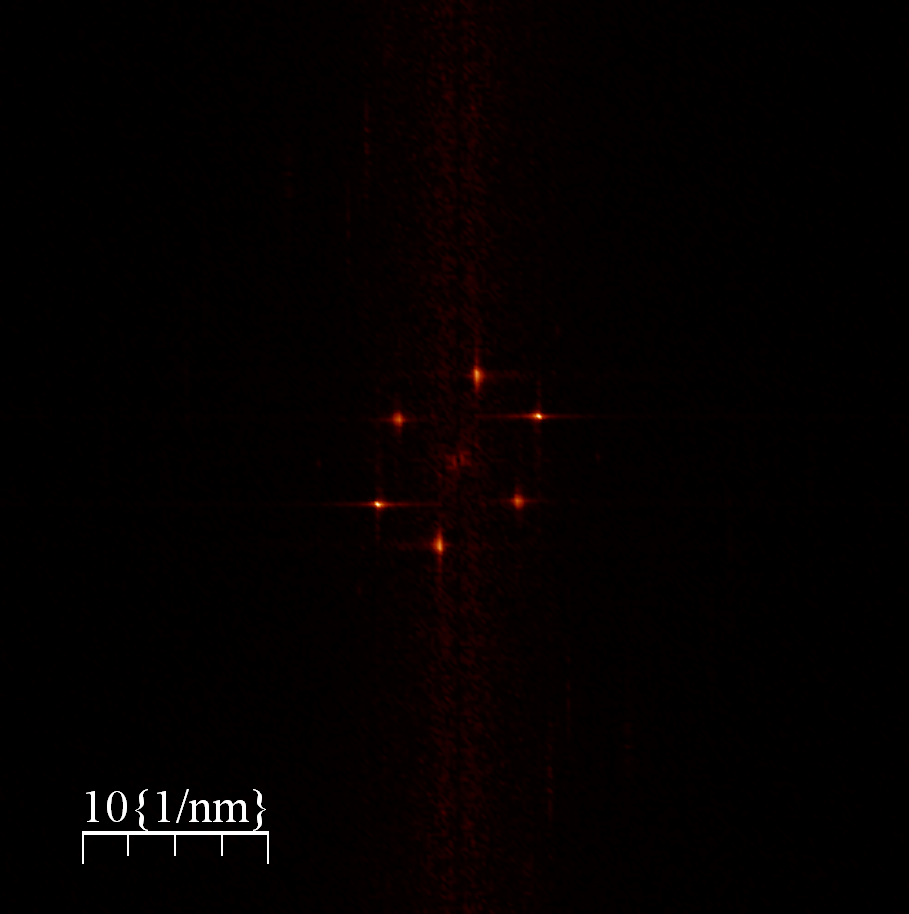
\includegraphics[width=0.5 \textwidth]{fft.png}
  \caption{2D-FFT}
\end{figure}

Man sieht hier eindeutig das triagonale Gitter als Intensitätspeaks der zwei
reziproken Gittervektoren vom Ursprung ausgehend im ersten Quadranten. Da nur
reele Werte transformiert wurden, ist das Bild punktsymmetrisch zum Ursprung.
Anhand der Beträge der Gittervektoren könnte man durch zurückrechnen in den
Realraum auch die Kantenlänge bestimmen. Da wir dies schon in Aufgabe d getan
haben, verweisen wir auf die Werte dort.

\subsection{Aufgabe f}

In Aufgabe b konnten wir leider keine Resultate erzielen. Dies liegt darin
begründet, dass die Präparation einer Probenspitze (a) experimentelles Geschick und
(b) Glück erfordert. Da die Präparation vom Tutor vorgenommen wurde, handelt es
sich selbstverständlich um (b).

Nach dem Ausfall des Geräts konnten wir leider kein stabiles Signal mehr
erzeugen. Dies liegt wahrscheinlich an (a), Einflüsse von (b) können nicht
ausgeschlossen werden.

Eine Diskussion der Fehler in d und e ist bereits dort ausführlich erfolgt,
ebenso wie Vergleiche mit dem Literaturwert.





\addcontentsline{toc}{section}{Literatur}
\bibliography{literatur}

\end{document}
